% fig_device_overview.tex - Cutaway diagram of psi-bubble propulsion vehicle
% Standalone compilation: pdflatex fig_device_overview.tex
% Also works with % fig_device_overview.tex - Cutaway diagram of psi-bubble propulsion vehicle
% Standalone compilation: pdflatex fig_device_overview.tex
% Also works with % fig_device_overview.tex - Cutaway diagram of psi-bubble propulsion vehicle
% Standalone compilation: pdflatex fig_device_overview.tex
% Also works with % fig_device_overview.tex - Cutaway diagram of psi-bubble propulsion vehicle
% Standalone compilation: pdflatex fig_device_overview.tex
% Also works with \input{figures/fig_device_overview} in main document
\documentclass[tikz,border=5pt]{standalone}
\usepackage{tikz}
\usepackage{amsmath}
\usetikzlibrary{decorations.markings,arrows.meta,patterns,calc,shadings,fadings}

\begin{document}
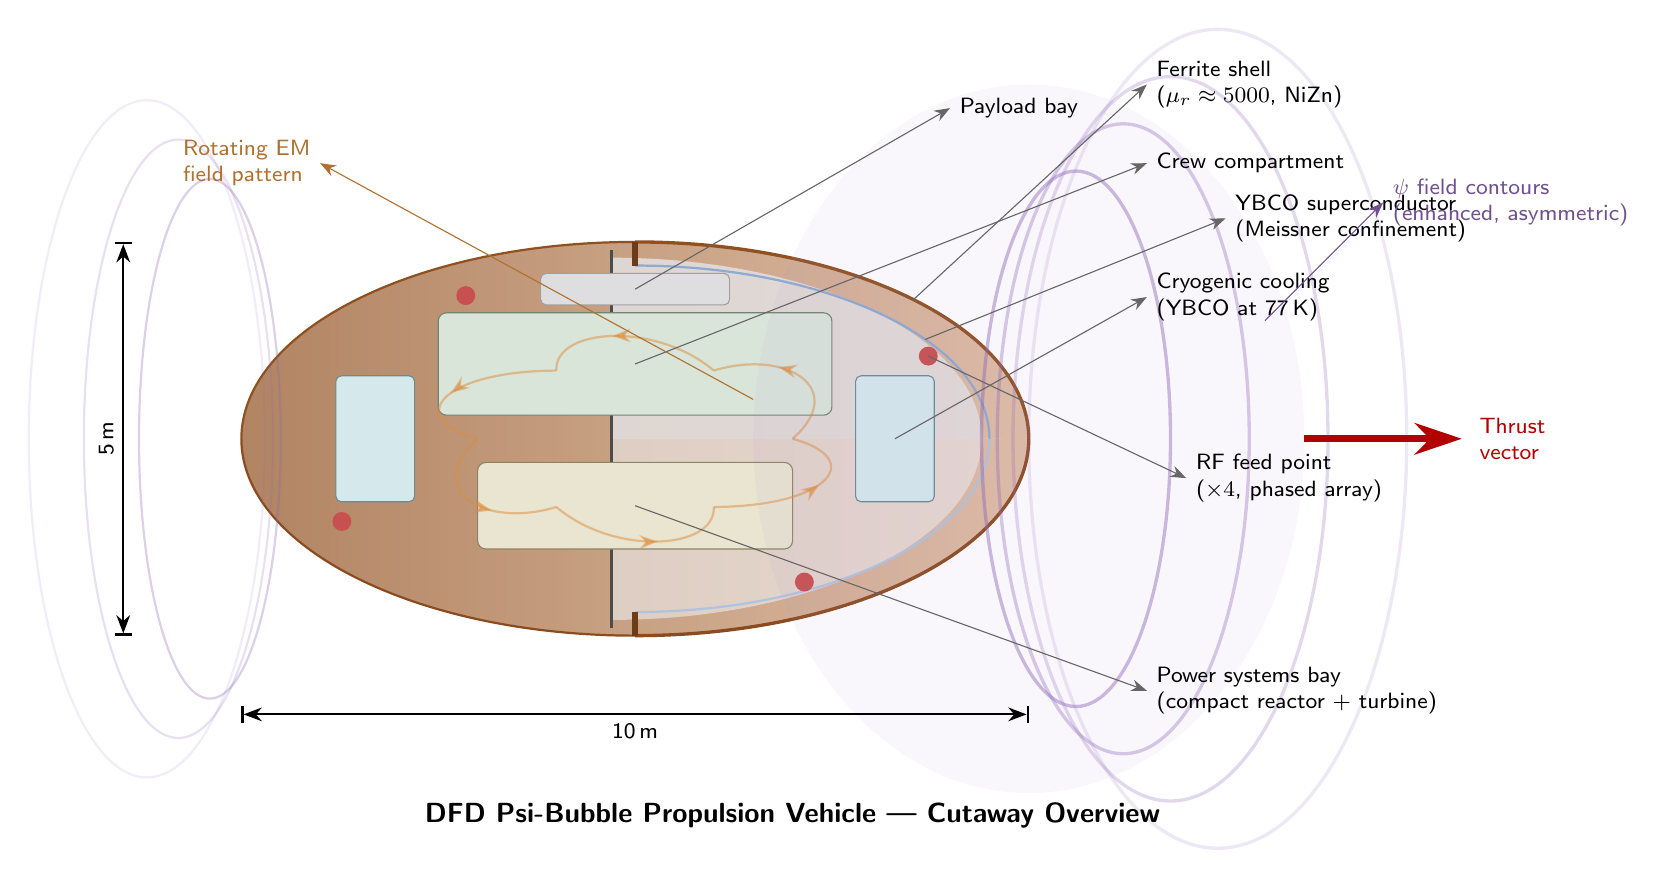
\begin{tikzpicture}[
    >=Stealth,
    every node/.style={font=\footnotesize},
    label node/.style={font=\footnotesize\sffamily, align=left},
    callout/.style={draw=black!60, thin, -{Stealth[length=2mm]}},
]

% --- Define colors ---
\definecolor{ferriteOrange}{RGB}{180,100,40}
\definecolor{ferriteDark}{RGB}{140,75,30}
\definecolor{scBlue}{RGB}{140,170,210}
\definecolor{scLight}{RGB}{180,200,230}
\definecolor{interiorGray}{RGB}{200,200,205}
\definecolor{crewGreen}{RGB}{160,190,160}
\definecolor{powerYellow}{RGB}{200,190,140}
\definecolor{cryoCyan}{RGB}{150,200,210}
\definecolor{psiPurple}{RGB}{140,100,180}
\definecolor{psiLight}{RGB}{180,150,220}
\definecolor{emRed}{RGB}{200,80,80}
\definecolor{emOrange}{RGB}{220,140,60}

% ============================================================
% VEHICLE BODY - oblate spheroid cutaway
% ============================================================

% --- Back half of shell (full) ---
\shade[left color=ferriteOrange!80!black, right color=ferriteOrange!60, opacity=0.7]
    (0,0) ellipse (5 and 2.5);

% --- Interior fill (visible through cutaway) ---
\fill[interiorGray!50, opacity=0.8]
    (-0.3,0) -- (-0.3,2.3) arc (90:0:4.7 and 2.3) -- (4.7,0) -- cycle;
\fill[interiorGray!30, opacity=0.6]
    (-0.3,0) -- (-0.3,-2.3) arc (-90:0:4.7 and 2.3) -- (4.7,0) -- cycle;

% --- Front cutaway shell (upper half) ---
\draw[ferriteOrange!80!black, very thick]
    (0,2.5) arc (90:0:5 and 2.5);
\draw[ferriteDark, very thick]
    (0,-2.5) arc (-90:0:5 and 2.5);

% --- Back shell outline ---
\draw[ferriteOrange!80!black, thick]
    (0,2.5) arc (90:180:5 and 2.5);
\draw[ferriteDark, thick]
    (0,-2.5) arc (-90:-180:5 and 2.5);

% --- Inner superconductor layer (visible in cutaway) ---
\draw[scBlue, thick]
    (0,2.2) arc (90:0:4.5 and 2.2);
\draw[scBlue!70, thick]
    (0,-2.2) arc (-90:0:4.5 and 2.2);

% --- Cutaway edge lines ---
\draw[black!70, thick] (-0.3,2.4) -- (-0.3,-2.4);
\draw[ferriteOrange!60!black, line width=2pt] (0,2.5) -- (0,2.2);
\draw[ferriteOrange!60!black, line width=2pt] (0,-2.5) -- (0,-2.2);

% ============================================================
% INTERIOR COMPARTMENTS
% ============================================================

% --- Crew compartment (center-upper) ---
\fill[crewGreen!40, rounded corners=3pt]
    (-2.5,0.3) rectangle (2.5,1.6);
\draw[crewGreen!70!black, rounded corners=3pt]
    (-2.5,0.3) rectangle (2.5,1.6);

% --- Power systems bay (center-lower) ---
\fill[powerYellow!40, rounded corners=3pt]
    (-2.0,-1.4) rectangle (2.0,-0.3);
\draw[powerYellow!70!black, rounded corners=3pt]
    (-2.0,-1.4) rectangle (2.0,-0.3);

% --- Cryogenics (flanking) ---
\fill[cryoCyan!40, rounded corners=2pt]
    (2.8,-0.8) rectangle (3.8,0.8);
\draw[cryoCyan!70!black, rounded corners=2pt]
    (2.8,-0.8) rectangle (3.8,0.8);

\fill[cryoCyan!40, rounded corners=2pt]
    (-3.8,-0.8) rectangle (-2.8,0.8);
\draw[cryoCyan!70!black, rounded corners=2pt]
    (-3.8,-0.8) rectangle (-2.8,0.8);

% --- Payload bay (upper-center) ---
\fill[interiorGray!60, rounded corners=2pt]
    (-1.2,1.7) rectangle (1.2,2.1);
\draw[interiorGray!80!black, rounded corners=2pt]
    (-1.2,1.7) rectangle (1.2,2.1);

% --- RF feed points (4 locations on inner shell) ---
\foreach \a in {30, 120, 210, 300} {
    \fill[emRed] ({4.3*cos(\a)},{2.1*sin(\a)}) circle (0.12);
}

% ============================================================
% EM FIELD LINES (rotating pattern inside shell)
% ============================================================
\foreach \i in {1,...,6} {
    \pgfmathsetmacro{\ang}{60*\i}
    \draw[emOrange, thick, opacity=0.5,
          decoration={markings, mark=at position 0.6 with {\arrow{>}}},
          postaction={decorate}]
        ({2.0*cos(\ang)},{1.0*sin(\ang)})
        .. controls ({3.0*cos(\ang+25)},{1.5*sin(\ang+25)})
        and ({3.0*cos(\ang+50)},{1.5*sin(\ang+50)})
        .. ({2.0*cos(\ang+60)},{1.0*sin(\ang+60)});
}

% ============================================================
% PSI FIELD CONTOURS (outside shell, asymmetric)
% ============================================================

% --- Weaker side (left) ---
\foreach \i/\op in {1/0.3, 2/0.2, 3/0.12} {
    \draw[psiPurple, thick, opacity=\op]
        ({-5-0.4*\i},0) ellipse ({0.6+0.3*\i} and {2.8+0.5*\i});
}

% --- Stronger side (right, thrust direction) ---
\foreach \i/\op in {1/0.45, 2/0.35, 3/0.25, 4/0.15} {
    \draw[psiPurple, very thick, opacity=\op]
        ({5+0.6*\i},0) ellipse ({0.8+0.4*\i} and {2.8+0.6*\i});
}

% --- Asymmetry gradient shading (right side stronger) ---
\fill[psiLight, opacity=0.08]
    (5,0) ellipse (3.5 and 4.5);

% ============================================================
% THRUST VECTOR
% ============================================================
\draw[-{Stealth[length=6mm, width=4mm]}, line width=2.5pt, red!70!black]
    (8.5,0) -- (10.5,0);
\node[label node, red!70!black, right] at (10.6,0) {Thrust\\vector};

% ============================================================
% LABELS AND CALLOUTS
% ============================================================

% Crew compartment
\draw[callout] (0,0.95) -- (6.5,3.5);
\node[label node, right] at (6.5,3.5) {Crew compartment};

% Power systems
\draw[callout] (0,-0.85) -- (6.5,-3.2);
\node[label node, right] at (6.5,-3.2) {Power systems bay\\(compact reactor + turbine)};

% Cryogenics
\draw[callout] (3.3,0) -- (6.5,1.8);
\node[label node, right] at (6.5,1.8) {Cryogenic cooling\\(YBCO at 77\,K)};

% Payload bay
\draw[callout] (0,1.9) -- (4,4.2);
\node[label node, right] at (4,4.2) {Payload bay};

% Ferrite shell
\draw[callout] ({5*cos(45)},{2.5*sin(45)}) -- (6.5,4.5);
\node[label node, right] at (6.5,4.5) {Ferrite shell\\($\mu_r \approx 5000$, NiZn)};

% Superconductor
\draw[callout] ({4.5*cos(35)},{2.2*sin(35)}) -- (7.5,2.8);
\node[label node, right] at (7.5,2.8) {YBCO superconductor\\(Meissner confinement)};

% RF feed points
\draw[callout] ({4.3*cos(30)},{2.1*sin(30)}) -- (7,-0.5);
\node[label node, right] at (7,-0.5) {RF feed point\\($\times 4$, phased array)};

% Psi field (right)
\draw[callout, psiPurple!80!black] (8,1.5) -- (9.5,3);
\node[label node, psiPurple!80!black, right] at (9.5,3) {$\psi$ field contours\\(enhanced, asymmetric)};

% EM field
\draw[callout, emOrange!80!black] (1.5,0.5) -- (-4,3.5);
\node[label node, emOrange!80!black, left] at (-4,3.5) {Rotating EM\\field pattern};

% ============================================================
% SCALE BAR
% ============================================================
\draw[black, thick, |<->|] (-5,-3.5) -- (5,-3.5);
\node[below, font=\footnotesize\sffamily] at (0,-3.5) {10\,m};

\draw[black, thick, |<->|] (-6.5,-2.5) -- (-6.5,2.5);
\node[left, font=\footnotesize\sffamily, rotate=90, anchor=south] at (-6.5,0) {5\,m};

% ============================================================
% TITLE
% ============================================================
\node[font=\normalsize\sffamily\bfseries, anchor=north] at (2,-4.5)
    {DFD Psi-Bubble Propulsion Vehicle --- Cutaway Overview};

\end{tikzpicture}
\end{document}
 in main document
\documentclass[tikz,border=5pt]{standalone}
\usepackage{tikz}
\usepackage{amsmath}
\usetikzlibrary{decorations.markings,arrows.meta,patterns,calc,shadings,fadings}

\begin{document}
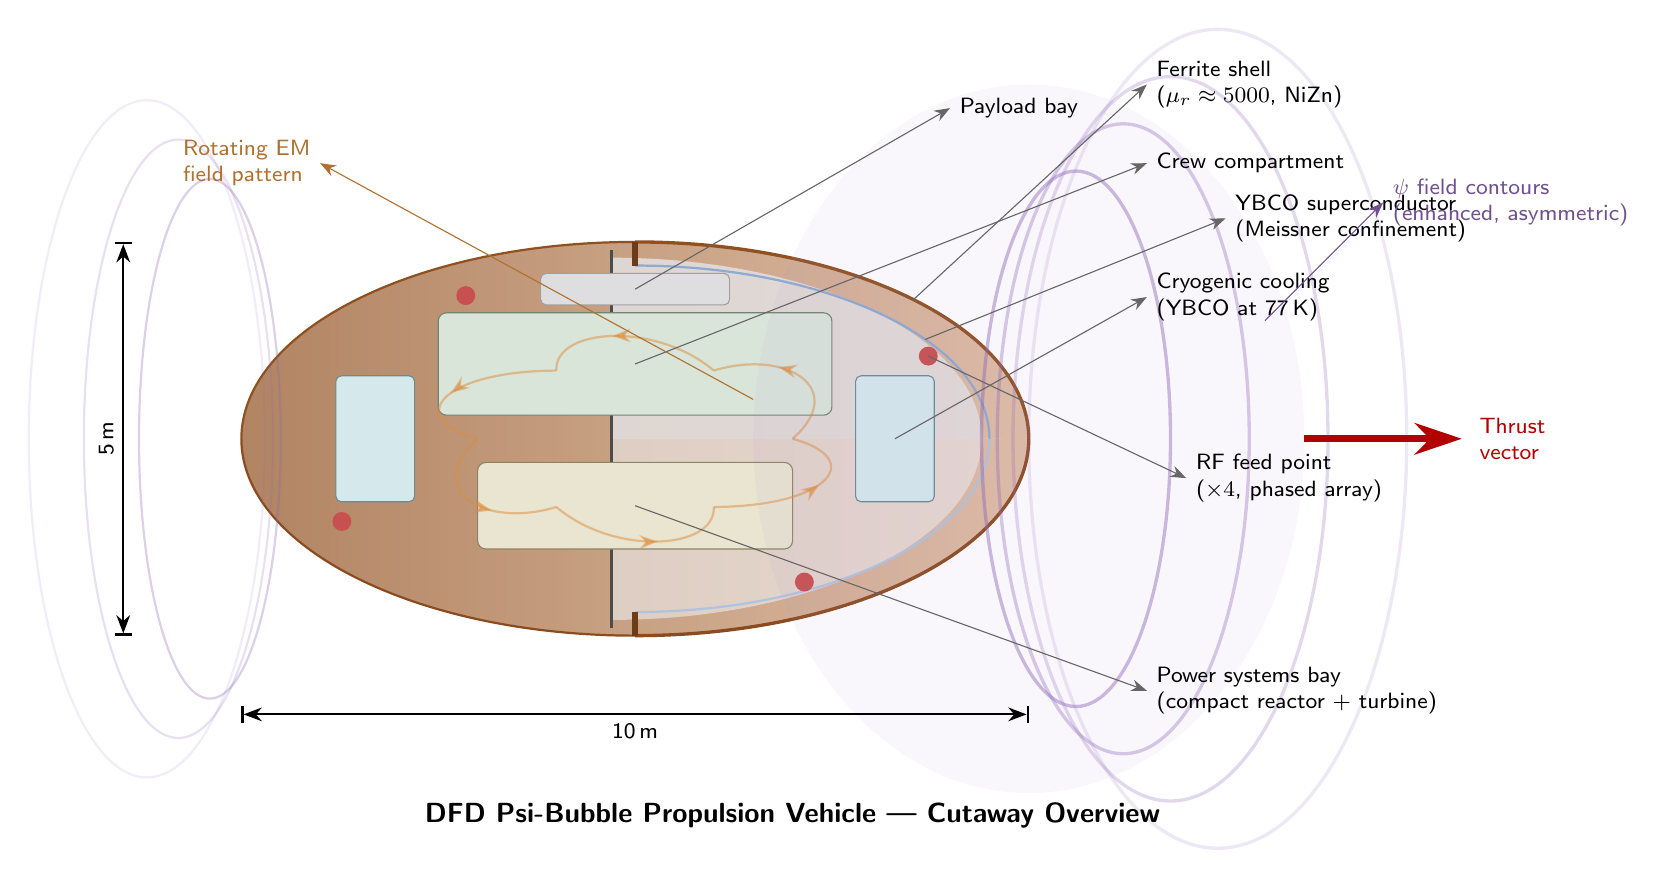
\begin{tikzpicture}[
    >=Stealth,
    every node/.style={font=\footnotesize},
    label node/.style={font=\footnotesize\sffamily, align=left},
    callout/.style={draw=black!60, thin, -{Stealth[length=2mm]}},
]

% --- Define colors ---
\definecolor{ferriteOrange}{RGB}{180,100,40}
\definecolor{ferriteDark}{RGB}{140,75,30}
\definecolor{scBlue}{RGB}{140,170,210}
\definecolor{scLight}{RGB}{180,200,230}
\definecolor{interiorGray}{RGB}{200,200,205}
\definecolor{crewGreen}{RGB}{160,190,160}
\definecolor{powerYellow}{RGB}{200,190,140}
\definecolor{cryoCyan}{RGB}{150,200,210}
\definecolor{psiPurple}{RGB}{140,100,180}
\definecolor{psiLight}{RGB}{180,150,220}
\definecolor{emRed}{RGB}{200,80,80}
\definecolor{emOrange}{RGB}{220,140,60}

% ============================================================
% VEHICLE BODY - oblate spheroid cutaway
% ============================================================

% --- Back half of shell (full) ---
\shade[left color=ferriteOrange!80!black, right color=ferriteOrange!60, opacity=0.7]
    (0,0) ellipse (5 and 2.5);

% --- Interior fill (visible through cutaway) ---
\fill[interiorGray!50, opacity=0.8]
    (-0.3,0) -- (-0.3,2.3) arc (90:0:4.7 and 2.3) -- (4.7,0) -- cycle;
\fill[interiorGray!30, opacity=0.6]
    (-0.3,0) -- (-0.3,-2.3) arc (-90:0:4.7 and 2.3) -- (4.7,0) -- cycle;

% --- Front cutaway shell (upper half) ---
\draw[ferriteOrange!80!black, very thick]
    (0,2.5) arc (90:0:5 and 2.5);
\draw[ferriteDark, very thick]
    (0,-2.5) arc (-90:0:5 and 2.5);

% --- Back shell outline ---
\draw[ferriteOrange!80!black, thick]
    (0,2.5) arc (90:180:5 and 2.5);
\draw[ferriteDark, thick]
    (0,-2.5) arc (-90:-180:5 and 2.5);

% --- Inner superconductor layer (visible in cutaway) ---
\draw[scBlue, thick]
    (0,2.2) arc (90:0:4.5 and 2.2);
\draw[scBlue!70, thick]
    (0,-2.2) arc (-90:0:4.5 and 2.2);

% --- Cutaway edge lines ---
\draw[black!70, thick] (-0.3,2.4) -- (-0.3,-2.4);
\draw[ferriteOrange!60!black, line width=2pt] (0,2.5) -- (0,2.2);
\draw[ferriteOrange!60!black, line width=2pt] (0,-2.5) -- (0,-2.2);

% ============================================================
% INTERIOR COMPARTMENTS
% ============================================================

% --- Crew compartment (center-upper) ---
\fill[crewGreen!40, rounded corners=3pt]
    (-2.5,0.3) rectangle (2.5,1.6);
\draw[crewGreen!70!black, rounded corners=3pt]
    (-2.5,0.3) rectangle (2.5,1.6);

% --- Power systems bay (center-lower) ---
\fill[powerYellow!40, rounded corners=3pt]
    (-2.0,-1.4) rectangle (2.0,-0.3);
\draw[powerYellow!70!black, rounded corners=3pt]
    (-2.0,-1.4) rectangle (2.0,-0.3);

% --- Cryogenics (flanking) ---
\fill[cryoCyan!40, rounded corners=2pt]
    (2.8,-0.8) rectangle (3.8,0.8);
\draw[cryoCyan!70!black, rounded corners=2pt]
    (2.8,-0.8) rectangle (3.8,0.8);

\fill[cryoCyan!40, rounded corners=2pt]
    (-3.8,-0.8) rectangle (-2.8,0.8);
\draw[cryoCyan!70!black, rounded corners=2pt]
    (-3.8,-0.8) rectangle (-2.8,0.8);

% --- Payload bay (upper-center) ---
\fill[interiorGray!60, rounded corners=2pt]
    (-1.2,1.7) rectangle (1.2,2.1);
\draw[interiorGray!80!black, rounded corners=2pt]
    (-1.2,1.7) rectangle (1.2,2.1);

% --- RF feed points (4 locations on inner shell) ---
\foreach \a in {30, 120, 210, 300} {
    \fill[emRed] ({4.3*cos(\a)},{2.1*sin(\a)}) circle (0.12);
}

% ============================================================
% EM FIELD LINES (rotating pattern inside shell)
% ============================================================
\foreach \i in {1,...,6} {
    \pgfmathsetmacro{\ang}{60*\i}
    \draw[emOrange, thick, opacity=0.5,
          decoration={markings, mark=at position 0.6 with {\arrow{>}}},
          postaction={decorate}]
        ({2.0*cos(\ang)},{1.0*sin(\ang)})
        .. controls ({3.0*cos(\ang+25)},{1.5*sin(\ang+25)})
        and ({3.0*cos(\ang+50)},{1.5*sin(\ang+50)})
        .. ({2.0*cos(\ang+60)},{1.0*sin(\ang+60)});
}

% ============================================================
% PSI FIELD CONTOURS (outside shell, asymmetric)
% ============================================================

% --- Weaker side (left) ---
\foreach \i/\op in {1/0.3, 2/0.2, 3/0.12} {
    \draw[psiPurple, thick, opacity=\op]
        ({-5-0.4*\i},0) ellipse ({0.6+0.3*\i} and {2.8+0.5*\i});
}

% --- Stronger side (right, thrust direction) ---
\foreach \i/\op in {1/0.45, 2/0.35, 3/0.25, 4/0.15} {
    \draw[psiPurple, very thick, opacity=\op]
        ({5+0.6*\i},0) ellipse ({0.8+0.4*\i} and {2.8+0.6*\i});
}

% --- Asymmetry gradient shading (right side stronger) ---
\fill[psiLight, opacity=0.08]
    (5,0) ellipse (3.5 and 4.5);

% ============================================================
% THRUST VECTOR
% ============================================================
\draw[-{Stealth[length=6mm, width=4mm]}, line width=2.5pt, red!70!black]
    (8.5,0) -- (10.5,0);
\node[label node, red!70!black, right] at (10.6,0) {Thrust\\vector};

% ============================================================
% LABELS AND CALLOUTS
% ============================================================

% Crew compartment
\draw[callout] (0,0.95) -- (6.5,3.5);
\node[label node, right] at (6.5,3.5) {Crew compartment};

% Power systems
\draw[callout] (0,-0.85) -- (6.5,-3.2);
\node[label node, right] at (6.5,-3.2) {Power systems bay\\(compact reactor + turbine)};

% Cryogenics
\draw[callout] (3.3,0) -- (6.5,1.8);
\node[label node, right] at (6.5,1.8) {Cryogenic cooling\\(YBCO at 77\,K)};

% Payload bay
\draw[callout] (0,1.9) -- (4,4.2);
\node[label node, right] at (4,4.2) {Payload bay};

% Ferrite shell
\draw[callout] ({5*cos(45)},{2.5*sin(45)}) -- (6.5,4.5);
\node[label node, right] at (6.5,4.5) {Ferrite shell\\($\mu_r \approx 5000$, NiZn)};

% Superconductor
\draw[callout] ({4.5*cos(35)},{2.2*sin(35)}) -- (7.5,2.8);
\node[label node, right] at (7.5,2.8) {YBCO superconductor\\(Meissner confinement)};

% RF feed points
\draw[callout] ({4.3*cos(30)},{2.1*sin(30)}) -- (7,-0.5);
\node[label node, right] at (7,-0.5) {RF feed point\\($\times 4$, phased array)};

% Psi field (right)
\draw[callout, psiPurple!80!black] (8,1.5) -- (9.5,3);
\node[label node, psiPurple!80!black, right] at (9.5,3) {$\psi$ field contours\\(enhanced, asymmetric)};

% EM field
\draw[callout, emOrange!80!black] (1.5,0.5) -- (-4,3.5);
\node[label node, emOrange!80!black, left] at (-4,3.5) {Rotating EM\\field pattern};

% ============================================================
% SCALE BAR
% ============================================================
\draw[black, thick, |<->|] (-5,-3.5) -- (5,-3.5);
\node[below, font=\footnotesize\sffamily] at (0,-3.5) {10\,m};

\draw[black, thick, |<->|] (-6.5,-2.5) -- (-6.5,2.5);
\node[left, font=\footnotesize\sffamily, rotate=90, anchor=south] at (-6.5,0) {5\,m};

% ============================================================
% TITLE
% ============================================================
\node[font=\normalsize\sffamily\bfseries, anchor=north] at (2,-4.5)
    {DFD Psi-Bubble Propulsion Vehicle --- Cutaway Overview};

\end{tikzpicture}
\end{document}
 in main document
\documentclass[tikz,border=5pt]{standalone}
\usepackage{tikz}
\usepackage{amsmath}
\usetikzlibrary{decorations.markings,arrows.meta,patterns,calc,shadings,fadings}

\begin{document}
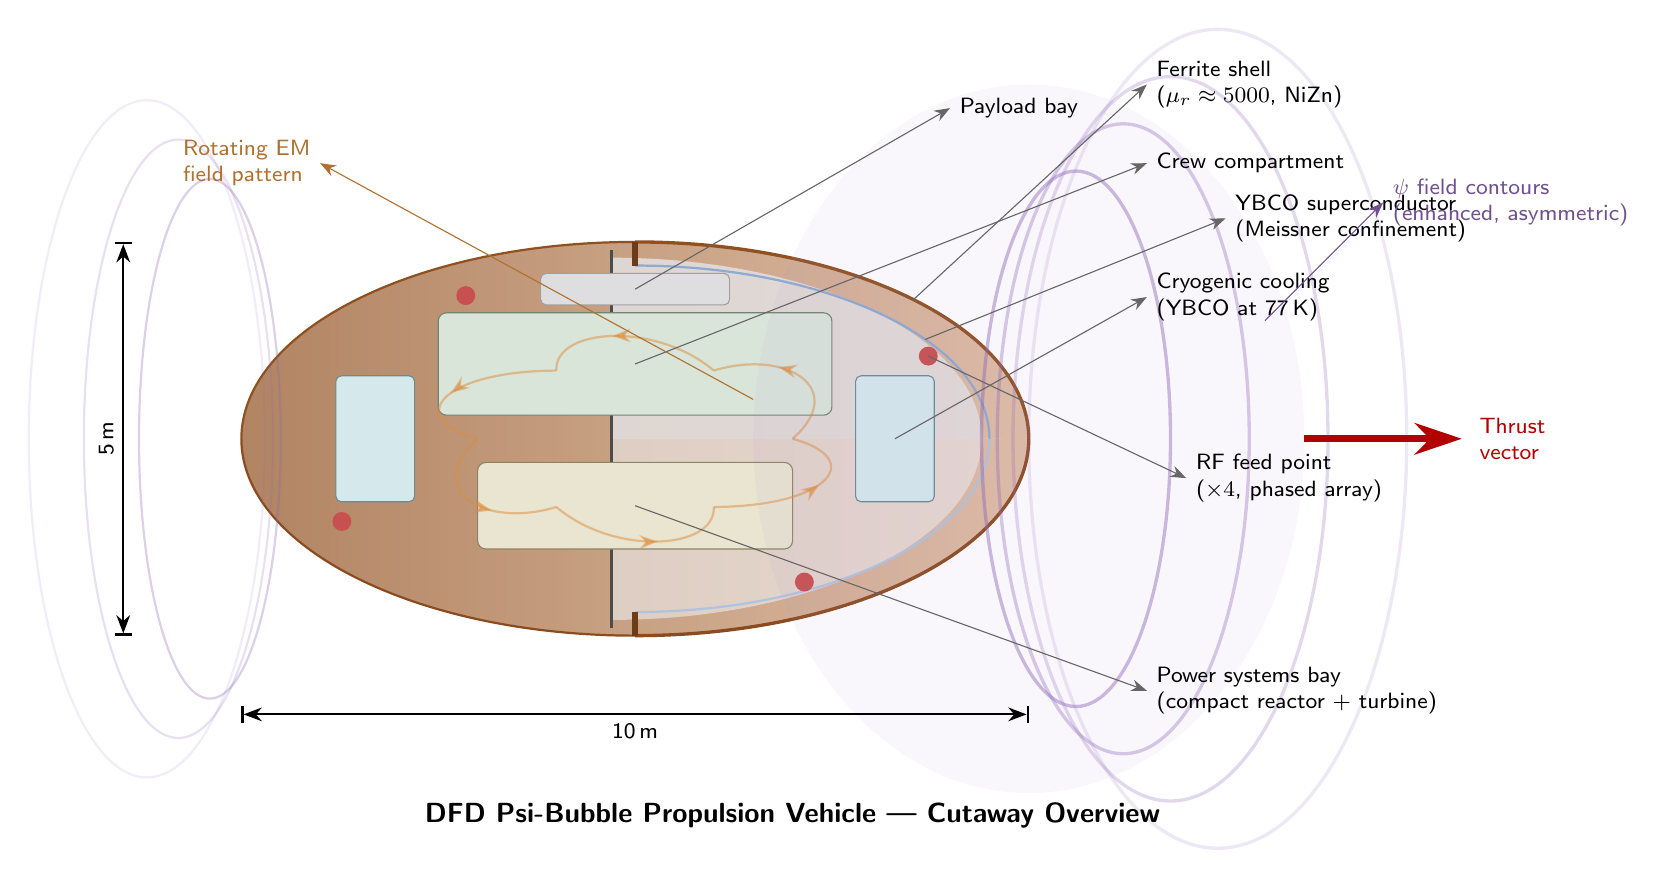
\begin{tikzpicture}[
    >=Stealth,
    every node/.style={font=\footnotesize},
    label node/.style={font=\footnotesize\sffamily, align=left},
    callout/.style={draw=black!60, thin, -{Stealth[length=2mm]}},
]

% --- Define colors ---
\definecolor{ferriteOrange}{RGB}{180,100,40}
\definecolor{ferriteDark}{RGB}{140,75,30}
\definecolor{scBlue}{RGB}{140,170,210}
\definecolor{scLight}{RGB}{180,200,230}
\definecolor{interiorGray}{RGB}{200,200,205}
\definecolor{crewGreen}{RGB}{160,190,160}
\definecolor{powerYellow}{RGB}{200,190,140}
\definecolor{cryoCyan}{RGB}{150,200,210}
\definecolor{psiPurple}{RGB}{140,100,180}
\definecolor{psiLight}{RGB}{180,150,220}
\definecolor{emRed}{RGB}{200,80,80}
\definecolor{emOrange}{RGB}{220,140,60}

% ============================================================
% VEHICLE BODY - oblate spheroid cutaway
% ============================================================

% --- Back half of shell (full) ---
\shade[left color=ferriteOrange!80!black, right color=ferriteOrange!60, opacity=0.7]
    (0,0) ellipse (5 and 2.5);

% --- Interior fill (visible through cutaway) ---
\fill[interiorGray!50, opacity=0.8]
    (-0.3,0) -- (-0.3,2.3) arc (90:0:4.7 and 2.3) -- (4.7,0) -- cycle;
\fill[interiorGray!30, opacity=0.6]
    (-0.3,0) -- (-0.3,-2.3) arc (-90:0:4.7 and 2.3) -- (4.7,0) -- cycle;

% --- Front cutaway shell (upper half) ---
\draw[ferriteOrange!80!black, very thick]
    (0,2.5) arc (90:0:5 and 2.5);
\draw[ferriteDark, very thick]
    (0,-2.5) arc (-90:0:5 and 2.5);

% --- Back shell outline ---
\draw[ferriteOrange!80!black, thick]
    (0,2.5) arc (90:180:5 and 2.5);
\draw[ferriteDark, thick]
    (0,-2.5) arc (-90:-180:5 and 2.5);

% --- Inner superconductor layer (visible in cutaway) ---
\draw[scBlue, thick]
    (0,2.2) arc (90:0:4.5 and 2.2);
\draw[scBlue!70, thick]
    (0,-2.2) arc (-90:0:4.5 and 2.2);

% --- Cutaway edge lines ---
\draw[black!70, thick] (-0.3,2.4) -- (-0.3,-2.4);
\draw[ferriteOrange!60!black, line width=2pt] (0,2.5) -- (0,2.2);
\draw[ferriteOrange!60!black, line width=2pt] (0,-2.5) -- (0,-2.2);

% ============================================================
% INTERIOR COMPARTMENTS
% ============================================================

% --- Crew compartment (center-upper) ---
\fill[crewGreen!40, rounded corners=3pt]
    (-2.5,0.3) rectangle (2.5,1.6);
\draw[crewGreen!70!black, rounded corners=3pt]
    (-2.5,0.3) rectangle (2.5,1.6);

% --- Power systems bay (center-lower) ---
\fill[powerYellow!40, rounded corners=3pt]
    (-2.0,-1.4) rectangle (2.0,-0.3);
\draw[powerYellow!70!black, rounded corners=3pt]
    (-2.0,-1.4) rectangle (2.0,-0.3);

% --- Cryogenics (flanking) ---
\fill[cryoCyan!40, rounded corners=2pt]
    (2.8,-0.8) rectangle (3.8,0.8);
\draw[cryoCyan!70!black, rounded corners=2pt]
    (2.8,-0.8) rectangle (3.8,0.8);

\fill[cryoCyan!40, rounded corners=2pt]
    (-3.8,-0.8) rectangle (-2.8,0.8);
\draw[cryoCyan!70!black, rounded corners=2pt]
    (-3.8,-0.8) rectangle (-2.8,0.8);

% --- Payload bay (upper-center) ---
\fill[interiorGray!60, rounded corners=2pt]
    (-1.2,1.7) rectangle (1.2,2.1);
\draw[interiorGray!80!black, rounded corners=2pt]
    (-1.2,1.7) rectangle (1.2,2.1);

% --- RF feed points (4 locations on inner shell) ---
\foreach \a in {30, 120, 210, 300} {
    \fill[emRed] ({4.3*cos(\a)},{2.1*sin(\a)}) circle (0.12);
}

% ============================================================
% EM FIELD LINES (rotating pattern inside shell)
% ============================================================
\foreach \i in {1,...,6} {
    \pgfmathsetmacro{\ang}{60*\i}
    \draw[emOrange, thick, opacity=0.5,
          decoration={markings, mark=at position 0.6 with {\arrow{>}}},
          postaction={decorate}]
        ({2.0*cos(\ang)},{1.0*sin(\ang)})
        .. controls ({3.0*cos(\ang+25)},{1.5*sin(\ang+25)})
        and ({3.0*cos(\ang+50)},{1.5*sin(\ang+50)})
        .. ({2.0*cos(\ang+60)},{1.0*sin(\ang+60)});
}

% ============================================================
% PSI FIELD CONTOURS (outside shell, asymmetric)
% ============================================================

% --- Weaker side (left) ---
\foreach \i/\op in {1/0.3, 2/0.2, 3/0.12} {
    \draw[psiPurple, thick, opacity=\op]
        ({-5-0.4*\i},0) ellipse ({0.6+0.3*\i} and {2.8+0.5*\i});
}

% --- Stronger side (right, thrust direction) ---
\foreach \i/\op in {1/0.45, 2/0.35, 3/0.25, 4/0.15} {
    \draw[psiPurple, very thick, opacity=\op]
        ({5+0.6*\i},0) ellipse ({0.8+0.4*\i} and {2.8+0.6*\i});
}

% --- Asymmetry gradient shading (right side stronger) ---
\fill[psiLight, opacity=0.08]
    (5,0) ellipse (3.5 and 4.5);

% ============================================================
% THRUST VECTOR
% ============================================================
\draw[-{Stealth[length=6mm, width=4mm]}, line width=2.5pt, red!70!black]
    (8.5,0) -- (10.5,0);
\node[label node, red!70!black, right] at (10.6,0) {Thrust\\vector};

% ============================================================
% LABELS AND CALLOUTS
% ============================================================

% Crew compartment
\draw[callout] (0,0.95) -- (6.5,3.5);
\node[label node, right] at (6.5,3.5) {Crew compartment};

% Power systems
\draw[callout] (0,-0.85) -- (6.5,-3.2);
\node[label node, right] at (6.5,-3.2) {Power systems bay\\(compact reactor + turbine)};

% Cryogenics
\draw[callout] (3.3,0) -- (6.5,1.8);
\node[label node, right] at (6.5,1.8) {Cryogenic cooling\\(YBCO at 77\,K)};

% Payload bay
\draw[callout] (0,1.9) -- (4,4.2);
\node[label node, right] at (4,4.2) {Payload bay};

% Ferrite shell
\draw[callout] ({5*cos(45)},{2.5*sin(45)}) -- (6.5,4.5);
\node[label node, right] at (6.5,4.5) {Ferrite shell\\($\mu_r \approx 5000$, NiZn)};

% Superconductor
\draw[callout] ({4.5*cos(35)},{2.2*sin(35)}) -- (7.5,2.8);
\node[label node, right] at (7.5,2.8) {YBCO superconductor\\(Meissner confinement)};

% RF feed points
\draw[callout] ({4.3*cos(30)},{2.1*sin(30)}) -- (7,-0.5);
\node[label node, right] at (7,-0.5) {RF feed point\\($\times 4$, phased array)};

% Psi field (right)
\draw[callout, psiPurple!80!black] (8,1.5) -- (9.5,3);
\node[label node, psiPurple!80!black, right] at (9.5,3) {$\psi$ field contours\\(enhanced, asymmetric)};

% EM field
\draw[callout, emOrange!80!black] (1.5,0.5) -- (-4,3.5);
\node[label node, emOrange!80!black, left] at (-4,3.5) {Rotating EM\\field pattern};

% ============================================================
% SCALE BAR
% ============================================================
\draw[black, thick, |<->|] (-5,-3.5) -- (5,-3.5);
\node[below, font=\footnotesize\sffamily] at (0,-3.5) {10\,m};

\draw[black, thick, |<->|] (-6.5,-2.5) -- (-6.5,2.5);
\node[left, font=\footnotesize\sffamily, rotate=90, anchor=south] at (-6.5,0) {5\,m};

% ============================================================
% TITLE
% ============================================================
\node[font=\normalsize\sffamily\bfseries, anchor=north] at (2,-4.5)
    {DFD Psi-Bubble Propulsion Vehicle --- Cutaway Overview};

\end{tikzpicture}
\end{document}
 in main document
\documentclass[tikz,border=5pt]{standalone}
\usepackage{tikz}
\usepackage{amsmath}
\usetikzlibrary{decorations.markings,arrows.meta,patterns,calc,shadings,fadings}

\begin{document}
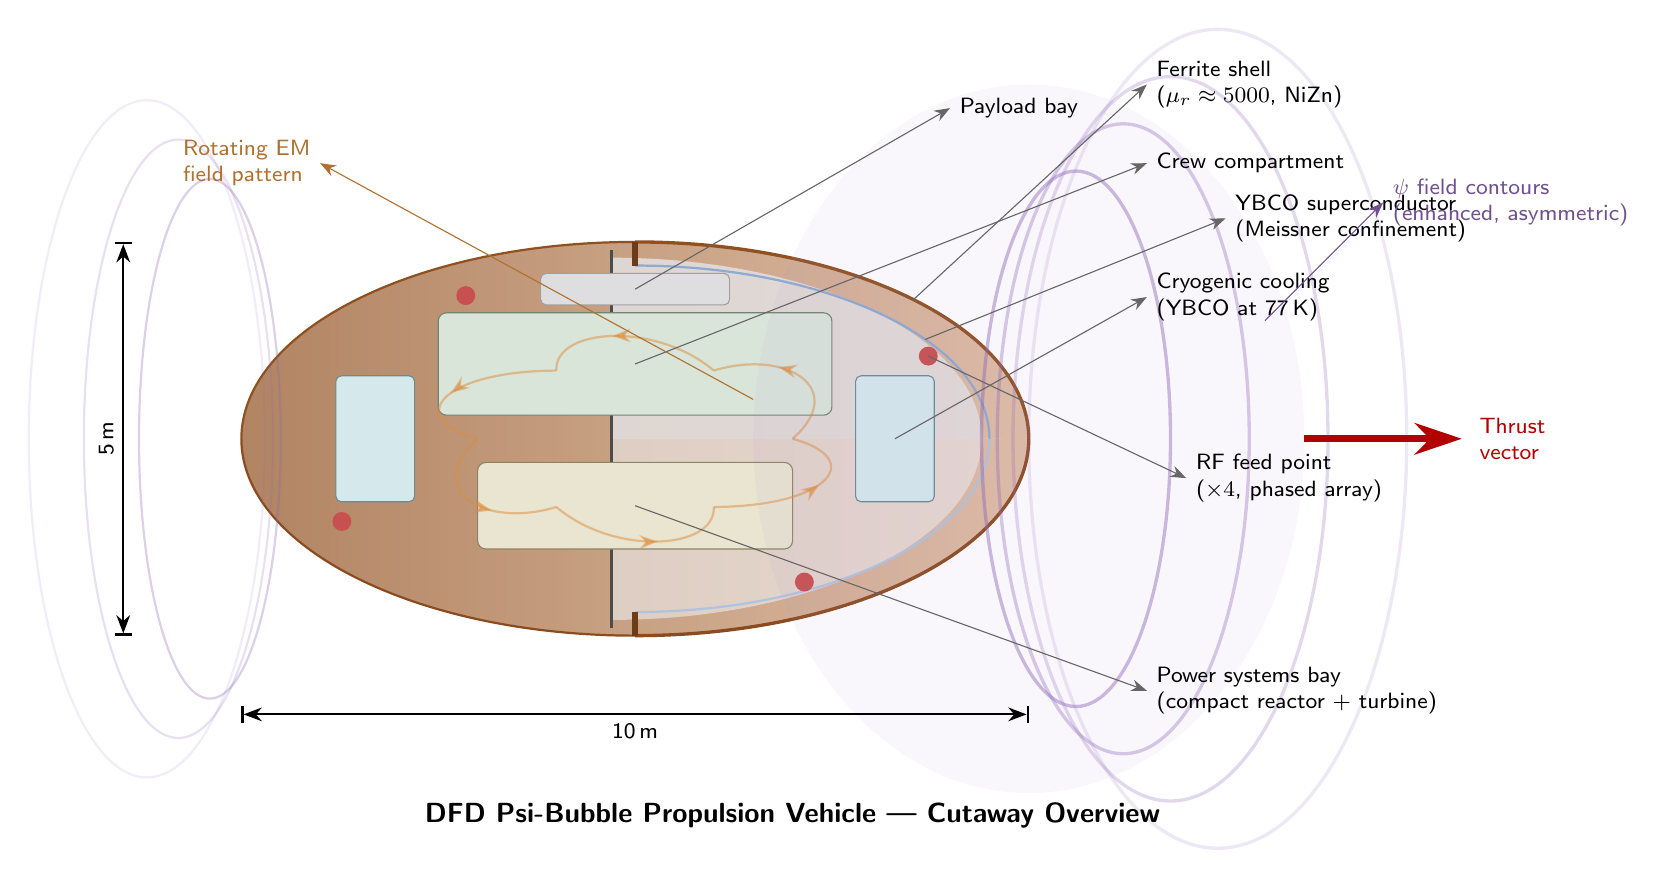
\begin{tikzpicture}[
    >=Stealth,
    every node/.style={font=\footnotesize},
    label node/.style={font=\footnotesize\sffamily, align=left},
    callout/.style={draw=black!60, thin, -{Stealth[length=2mm]}},
]

% --- Define colors ---
\definecolor{ferriteOrange}{RGB}{180,100,40}
\definecolor{ferriteDark}{RGB}{140,75,30}
\definecolor{scBlue}{RGB}{140,170,210}
\definecolor{scLight}{RGB}{180,200,230}
\definecolor{interiorGray}{RGB}{200,200,205}
\definecolor{crewGreen}{RGB}{160,190,160}
\definecolor{powerYellow}{RGB}{200,190,140}
\definecolor{cryoCyan}{RGB}{150,200,210}
\definecolor{psiPurple}{RGB}{140,100,180}
\definecolor{psiLight}{RGB}{180,150,220}
\definecolor{emRed}{RGB}{200,80,80}
\definecolor{emOrange}{RGB}{220,140,60}

% ============================================================
% VEHICLE BODY - oblate spheroid cutaway
% ============================================================

% --- Back half of shell (full) ---
\shade[left color=ferriteOrange!80!black, right color=ferriteOrange!60, opacity=0.7]
    (0,0) ellipse (5 and 2.5);

% --- Interior fill (visible through cutaway) ---
\fill[interiorGray!50, opacity=0.8]
    (-0.3,0) -- (-0.3,2.3) arc (90:0:4.7 and 2.3) -- (4.7,0) -- cycle;
\fill[interiorGray!30, opacity=0.6]
    (-0.3,0) -- (-0.3,-2.3) arc (-90:0:4.7 and 2.3) -- (4.7,0) -- cycle;

% --- Front cutaway shell (upper half) ---
\draw[ferriteOrange!80!black, very thick]
    (0,2.5) arc (90:0:5 and 2.5);
\draw[ferriteDark, very thick]
    (0,-2.5) arc (-90:0:5 and 2.5);

% --- Back shell outline ---
\draw[ferriteOrange!80!black, thick]
    (0,2.5) arc (90:180:5 and 2.5);
\draw[ferriteDark, thick]
    (0,-2.5) arc (-90:-180:5 and 2.5);

% --- Inner superconductor layer (visible in cutaway) ---
\draw[scBlue, thick]
    (0,2.2) arc (90:0:4.5 and 2.2);
\draw[scBlue!70, thick]
    (0,-2.2) arc (-90:0:4.5 and 2.2);

% --- Cutaway edge lines ---
\draw[black!70, thick] (-0.3,2.4) -- (-0.3,-2.4);
\draw[ferriteOrange!60!black, line width=2pt] (0,2.5) -- (0,2.2);
\draw[ferriteOrange!60!black, line width=2pt] (0,-2.5) -- (0,-2.2);

% ============================================================
% INTERIOR COMPARTMENTS
% ============================================================

% --- Crew compartment (center-upper) ---
\fill[crewGreen!40, rounded corners=3pt]
    (-2.5,0.3) rectangle (2.5,1.6);
\draw[crewGreen!70!black, rounded corners=3pt]
    (-2.5,0.3) rectangle (2.5,1.6);

% --- Power systems bay (center-lower) ---
\fill[powerYellow!40, rounded corners=3pt]
    (-2.0,-1.4) rectangle (2.0,-0.3);
\draw[powerYellow!70!black, rounded corners=3pt]
    (-2.0,-1.4) rectangle (2.0,-0.3);

% --- Cryogenics (flanking) ---
\fill[cryoCyan!40, rounded corners=2pt]
    (2.8,-0.8) rectangle (3.8,0.8);
\draw[cryoCyan!70!black, rounded corners=2pt]
    (2.8,-0.8) rectangle (3.8,0.8);

\fill[cryoCyan!40, rounded corners=2pt]
    (-3.8,-0.8) rectangle (-2.8,0.8);
\draw[cryoCyan!70!black, rounded corners=2pt]
    (-3.8,-0.8) rectangle (-2.8,0.8);

% --- Payload bay (upper-center) ---
\fill[interiorGray!60, rounded corners=2pt]
    (-1.2,1.7) rectangle (1.2,2.1);
\draw[interiorGray!80!black, rounded corners=2pt]
    (-1.2,1.7) rectangle (1.2,2.1);

% --- RF feed points (4 locations on inner shell) ---
\foreach \a in {30, 120, 210, 300} {
    \fill[emRed] ({4.3*cos(\a)},{2.1*sin(\a)}) circle (0.12);
}

% ============================================================
% EM FIELD LINES (rotating pattern inside shell)
% ============================================================
\foreach \i in {1,...,6} {
    \pgfmathsetmacro{\ang}{60*\i}
    \draw[emOrange, thick, opacity=0.5,
          decoration={markings, mark=at position 0.6 with {\arrow{>}}},
          postaction={decorate}]
        ({2.0*cos(\ang)},{1.0*sin(\ang)})
        .. controls ({3.0*cos(\ang+25)},{1.5*sin(\ang+25)})
        and ({3.0*cos(\ang+50)},{1.5*sin(\ang+50)})
        .. ({2.0*cos(\ang+60)},{1.0*sin(\ang+60)});
}

% ============================================================
% PSI FIELD CONTOURS (outside shell, asymmetric)
% ============================================================

% --- Weaker side (left) ---
\foreach \i/\op in {1/0.3, 2/0.2, 3/0.12} {
    \draw[psiPurple, thick, opacity=\op]
        ({-5-0.4*\i},0) ellipse ({0.6+0.3*\i} and {2.8+0.5*\i});
}

% --- Stronger side (right, thrust direction) ---
\foreach \i/\op in {1/0.45, 2/0.35, 3/0.25, 4/0.15} {
    \draw[psiPurple, very thick, opacity=\op]
        ({5+0.6*\i},0) ellipse ({0.8+0.4*\i} and {2.8+0.6*\i});
}

% --- Asymmetry gradient shading (right side stronger) ---
\fill[psiLight, opacity=0.08]
    (5,0) ellipse (3.5 and 4.5);

% ============================================================
% THRUST VECTOR
% ============================================================
\draw[-{Stealth[length=6mm, width=4mm]}, line width=2.5pt, red!70!black]
    (8.5,0) -- (10.5,0);
\node[label node, red!70!black, right] at (10.6,0) {Thrust\\vector};

% ============================================================
% LABELS AND CALLOUTS
% ============================================================

% Crew compartment
\draw[callout] (0,0.95) -- (6.5,3.5);
\node[label node, right] at (6.5,3.5) {Crew compartment};

% Power systems
\draw[callout] (0,-0.85) -- (6.5,-3.2);
\node[label node, right] at (6.5,-3.2) {Power systems bay\\(compact reactor + turbine)};

% Cryogenics
\draw[callout] (3.3,0) -- (6.5,1.8);
\node[label node, right] at (6.5,1.8) {Cryogenic cooling\\(YBCO at 77\,K)};

% Payload bay
\draw[callout] (0,1.9) -- (4,4.2);
\node[label node, right] at (4,4.2) {Payload bay};

% Ferrite shell
\draw[callout] ({5*cos(45)},{2.5*sin(45)}) -- (6.5,4.5);
\node[label node, right] at (6.5,4.5) {Ferrite shell\\($\mu_r \approx 5000$, NiZn)};

% Superconductor
\draw[callout] ({4.5*cos(35)},{2.2*sin(35)}) -- (7.5,2.8);
\node[label node, right] at (7.5,2.8) {YBCO superconductor\\(Meissner confinement)};

% RF feed points
\draw[callout] ({4.3*cos(30)},{2.1*sin(30)}) -- (7,-0.5);
\node[label node, right] at (7,-0.5) {RF feed point\\($\times 4$, phased array)};

% Psi field (right)
\draw[callout, psiPurple!80!black] (8,1.5) -- (9.5,3);
\node[label node, psiPurple!80!black, right] at (9.5,3) {$\psi$ field contours\\(enhanced, asymmetric)};

% EM field
\draw[callout, emOrange!80!black] (1.5,0.5) -- (-4,3.5);
\node[label node, emOrange!80!black, left] at (-4,3.5) {Rotating EM\\field pattern};

% ============================================================
% SCALE BAR
% ============================================================
\draw[black, thick, |<->|] (-5,-3.5) -- (5,-3.5);
\node[below, font=\footnotesize\sffamily] at (0,-3.5) {10\,m};

\draw[black, thick, |<->|] (-6.5,-2.5) -- (-6.5,2.5);
\node[left, font=\footnotesize\sffamily, rotate=90, anchor=south] at (-6.5,0) {5\,m};

% ============================================================
% TITLE
% ============================================================
\node[font=\normalsize\sffamily\bfseries, anchor=north] at (2,-4.5)
    {DFD Psi-Bubble Propulsion Vehicle --- Cutaway Overview};

\end{tikzpicture}
\end{document}
